\documentclass[11pt]{article}

\usepackage[margin=1in]{geometry}

\usepackage{graphicx}
\usepackage{tabularx}

\usepackage{needspace}
\usepackage{longtable}

\usepackage[colorlinks=true, linkcolor=blue, urlcolor=blue, citecolor=blue]{hyperref}

% ---------- entorno CV block ----------
\newenvironment{cvblock}[3]
{
\noindent
\begin{longtable}{p{#1}  >{\raggedright\arraybackslash}p{#2} p{#3}}
}
{
\end{longtable}
}

% ---------- macro auxiliar para filas ----------
\newcommand{\cventry}[3]{\textbf{#1} & #2 & #3 \\ }

\newcommand{\paper}[4]{\small #2, “\textit{#1}”, \href{https://arxiv.org/abs/#3}{[arXiv:#3]} #4 \vspace{0.2cm}}
\newcommand{\talk}[2]{\small “\textit{#1}”, #2\vspace{0.2cm}}
\newcommand{\event}[2]{\small “\textit{#1}”, #2\vspace{0.2cm}}

%=============================================================================================================================
%=============================================================================================================================
\begin{document}

\begin{center}
\begin{minipage}{0.7\textwidth}
	{\textbf{\LARGE Marcelo Andrés Oyarzo Catalán}}	\vspace{0.4cm}
\\
IGFAE, Universidade de Santiago de Compostela\\
marceloandres.oyarzo@usc.cl\\
\url{https://orcid.org/0009-0003-4370-0568}\\
\url{https://moyarzoca.github.io/}
\end{minipage}
\begin{minipage}{0.25\textwidth}
\raggedleft
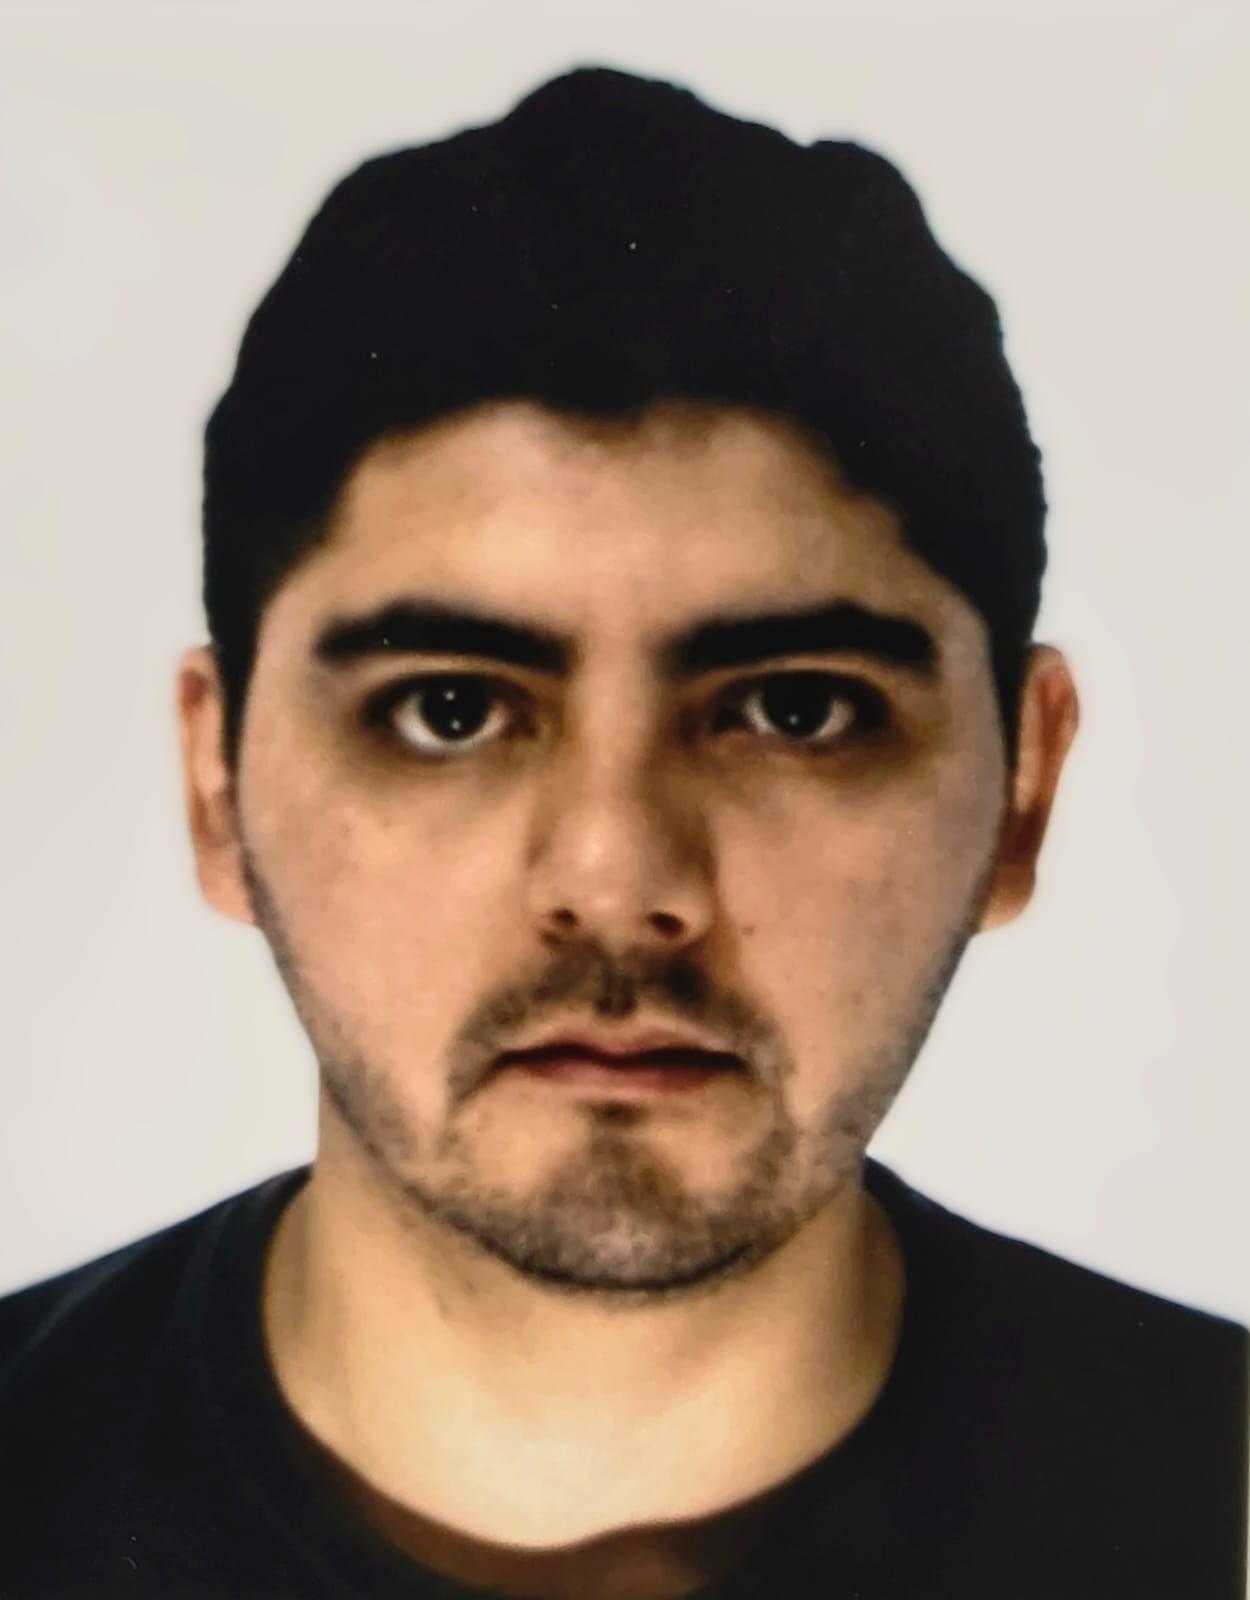
\includegraphics[width=3cm]{photo.jpg} % Replace with your file name
\end{minipage}
\end{center}

\begin{cvblock}{3cm}{0cm}{13cm}
\cventry{About me}{}{A theoretical physicist and postdoctoral researcher at IGFA, working on gravity and related aspects of quantum field theory.}
\end{cvblock}

\begin{cvblock}{3cm}{3cm}{10cm}
\cventry{Employment}{2026-present}{Postdoctoral Researcher, IGFAE Universidade de Santiago de Compostela}
\end{cvblock}


\begin{cvblock}{2.5cm}{0cm}{13cm}
\cventry{Education}{}{\textbf{PhD in Physics} \hfill 2022--2025}
	\cventry{}{}{Double degree at \textit{Universidad de Concepción, Chile} \& \textit{Politecnico di Torino, Italy.}}
	\cventry{}{}{Thesis: Black holes and Solitons in string theory}
	\cventry{}{}{Advisors: Andrés Anabalón, Julio Oliva, Mario Trigiante.}\\
\cventry{}{}{\textbf{Master in Physics} \hfill 2020--2022}
	\cventry{}{}{\textit{Universidad de Concepción, Chile}}
	\cventry{}{}{Thesis: Black holes and solitons in supergravity and their exact scalar (quasi) normal modes}
	\cventry{}{}{Advisors: Julio Oliva, Fabrizio Canfora}\\
\cventry{}{}{\textbf{Bachelor in physics} \hfill 2016--2020}
	\cventry{}{}{\textit{Universidad de Concepción, Chile}}
\end{cvblock}


\begin{cvblock}{2.5cm}{8cm}{3cm}
		\cventry{Grants}{FONDECYT regular 1262452}{co-investigador}
		\cventry{}{FONDECYT regular 1250133}{co-investigador}
		\cventry{}{FONDECYT regular 11200025}{personal técnico}
		\cventry{}{FONDECYT iniciación 11221063}{personal técnico}
\end{cvblock}


\begin{cvblock}{2.5cm}{0cm}{13cm}
\cventry{Fellowships}{}{\textbf{PhD Fellowship (cotutelle)} \hfill Mar. 7, 2022 – Oct. 3, 2024}
	\cventry{}{}{\textit{Universidad de Concepción, Chile / Politecnico di Torino, Italy} — Funded by Agencia Nacional de Investigación y Desarrollo (ANID).}
\cventry{}{}{\textbf{Master Fellowship} \hfill Mar. 30, 2020 – Mar. 1, 2022}
	\cventry{}{}{\textit{Universidad de Concepción, Chile} — Funded by Agencia Nacional de Investigación y Desarrollo (ANID).}
\end{cvblock}

\begin{cvblock}{2.8cm}{1cm}{13cm}
	\cventry{Peer Review}{\small 2025}{\event{Annals of Physics}{Reviewer, Elsevier.}}
\end{cvblock}

\begin{cvblock}{2.5cm}{2cm}{13cm}
\cventry{Teaching}{\small 2022}{Classical Mechanics.}
	\cventry{Assistant}{\small 2021}{Statistical Physics.}
	\cventry{}{\small 2020}{Introduction to Particle Physics and Quantum Field Theory.}
	\cventry{}{\small 2018}{Differential and Integral Calculus.}
	\cventry{}{\small 2017}{Electromagnetism for Engineering Students.}
\end{cvblock}


\begin{cvblock}{2.5cm}{2cm}{13cm}
	\cventry{Organization}{\small Jul. 2021}{\event{School on Holography and Supergravity}{Online School.}}
	\cventry{of Events}{\small Jan. 2021}{\event{School on Classical and Quantum Black Holes}{at Universidad de Concepción.}}
	\cventry{}{\small 2020-2021}{\event{Gravity Group Seminar at UdeC }{Online seminars.}}
\end{cvblock}



\section*{Publications}

\begin{cvblock}{1.8cm}{0cm}{13cm}
	\cventry{Preprints}{}{\paper{Logarithmic corrections to the entropy of near-extremal black holes in Einstein-Gauss-Bonnet}{Alejandro Alvarado, Andres Anabalon, Mariano Chernicoff, Julio Oliva, Marcelo Oyarzo, Gabriel Ortega, Jorge Urbina}{2603.24939}{} }

	\cventry{}{}{\paper{Moduli space of N=4 Super Yang-Mills from AdS/CFT}{Andrés Anabalón, Horatiu Nastase, Carlos Nunez, Marcelo Oyarzo, Ricardo Stuardo}{2603.18141}{}}

	\cventry{Published}{}{\paper{Warped-AdS3 Near-Horizon Geometries From TsT Transformations}{Stefano Maurelli, Ruggero Noris, Marcelo Oyarzo, Mario Trigiante}{2512.01770}{JHEP 03 (2026) 186}}

	\cventry{}{}{\paper{(Iso)spin from Isospin in Top-Down Holography}{Marcelo Oyarzo, Ricardo Stuardo}{2512.02120}{Accepted for publication in JHEP, 2025}}

	\cventry{}{}{\paper{Tessellation Groups, Harmonic Analysis on Non-compact Symmetric Spaces and the Heat Kernel in view of Cartan Convolutional Neural Networks}{Pietro Fré, Federico Milanesio, Marcelo Oyarzo, Matteo Santoro, Mario Trigiante}{2508.16015}{Accepted for publication in Fortschritte der Physik, 2025}}

	\cventry{}{}{\paper{Supersymmetric warped solutions from Type IIB orientifold reduction}{Stefano Maurelli, Ruggero Noris, Marcelo Oyarzo, Henning Samtleben, Mario Trigiante}{2504.16822}{JHEP 08 (2025) 013, 2025}}

	\cventry{}{}{\paper{The instability of low-temperature black holes in gauged N = 8 supergravity}{Andrés Anabalón, Stefano Maurelli, Marcelo Oyarzo, Mario Trigiante}{2411.09454}{JHEP 03 (2025) 201, 2024}}

	\cventry{}{}{\paper{Existence of a supersymmetric extension of the gauged nonlinear $\Sigma$ model and the transition from integrability to chaos}{Fabrizio Canfora, Nicolás Grandi, Marcelo Oyarzo}{2411.04245}{Phys.Rev.D 111 (2025) 11, 114026, 2024}}

	\cventry{}{}{\paper{Overflying nilpotent horizons}{Jose Figueroa, Gaston Giribet, Anibal Neira-Gallegos, Julio Oliva, Marcelo Oyarzo}{2404.18378}{Eur.Phys.J.C 84 (2024) 11, 1215, 2024}}

	\cventry{}{}{\paper{Black hole shadows of $\alpha'$-corrected black holes}{Felipe Agurto-Sepúlveda, Julio Oliva, Marcelo Oyarzo, Dominik R. G. Schleicher}{2404.12811}{Phys.Rev.D 110 (2024) 2, 2024}}

	\cventry{}{}{\paper{Supersymmetric AdS solitons and the interconnection of different vacua of N = 4 Super Yang-Mills}{Andrés Anabalón, Horatiu Nastase, Marcelo Oyarzo}{2402.18482}{JHEP 05 (2024) 217, 2024}}

	\cventry{}{}{\paper{Mixing “Magnetic” and “Electric” Ehlers–Harrison transformations: the electromagnetic swirling spacetime and novel type I backgrounds}{José Barrientos, Adolfo Cisterna, Ivan Kolář, Keanu Müller, Marcelo Oyarzo, Konstantinos Pallikaris}{2401.02924}{Eur.Phys.J.C 84 (2024) 7, 724, 2024}}

	\cventry{}{}{\paper{Confinement and D5-branes}{Carlos Nunez, Marcelo Oyarzo, Ricardo Stuardo}{2311.17998}{JHEP 03 (2024) 080, 2023}}

	\cventry{}{}{\paper{Exact oscillations and chaos on a non-Abelian coil}{Fabrizio Canfora, Nicolas Grandi, Marcelo Oyarzo, Julio Oliva}{2309.04915}{Nucl.Phys.B 1004 (2024) 116553, 2023}}

	\cventry{}{}{\paper{Confinement in (1 + 1) dimensions: a holographic perspective from I-branes}{Carlos Nunez, Marcelo Oyarzo, Ricardo Stuardo}{2307.04783}{JHEP 09 (2023) 201, 2023}}

	\cventry{}{}{\paper{$R^2$ corrections to the black string instability and the boosted black string}{Carla Henríquez-Báez, Julio Oliva, Marcelo Oyarzo, Marcel Yáñez-Reyes}{2212.07296}{Phys.Rev.D 107 (2023) 4, 2022}}

	\cventry{}{}{\paper{Slowly rotating and accelerating $\alpha'$-corrected black holes in four and higher dimensions}{Felipe Agurto-Sepúlveda, Mariano Chernicoff, Gaston Giribet, Julio Oliva, Marcelo Oyarzo}{2207.13214}{Phys.Rev.D 107 (2023) 8, 2022}}

	\cventry{}{}{\paper{Gravitational instantons with conformally coupled scalar fields}{José Barrientos, Adolfo Cisterna, Cristóbal Corral, Marcelo Oyarzo}{2202.13854}{JHEP 05 (2022) 110, 2022}}

	\cventry{}{}{\paper{Exact scalar (quasi-)normal modes of black holes and solitons in gauged SUGRA}{Monserrat Aguayo, Ankai Hernández, José Mena, Julio Oliva, Marcelo Oyarzo}{2101.00438}{JHEP 07 (2022) 021, 2022}}

	\cventry{}{}{\paper{New BPS solitons in N = 4 gauged supergravity and black holes in Einstein-Yang-Mills-dilaton theory}{Fabrizio Canfora, Julio Oliva, Marcelo Oyarzo}{2111.11915}{JHEP 02 (2022) 057, 2021}}

	\cventry{}{}{\paper{Quadratic gravity and conformally coupled scalar fields}{Nicolas Caceres, Jose Figueroa, Julio Oliva, Marcelo Oyarzo, Ricardo Stuardo}{2001.01478}{JHEP 04 (2020) 157, 2020}}
	
	\cventry{Conference papers}{}{\paper{Deforming $\mathrm{AdS}_3 \times S^3 \times T^4$ in Type IIB Supergravity}{Stefano Maurelli, Ruggero Noris, Marcelo Oyarzo, Mario Trigiante}{2604.26854}{, PoS CORFU2025 (2026) XXX, XXXX} }

	\cventry{}{}{\paper{On U-Folds and Their Construction}{Stefano Maurelli, Ruggero Noris, Marcelo Oyarzo, Mario Trigiante}{2504.16822}{, PoS CORFU2024 (2025) 178, 2025} }

	\cventry{}{}{\paper{Slowly rotating black holes modeled by Solv geometries }{Jose Figueroa, Marcelo Oyarzo}{2102.02328}{22nd Chilean Physics Symposium 2020, 2021}}
\end{cvblock}

\section*{Talks}
\begin{cvblock}{0cm}{2.3cm}{13cm}
	\noindent \cventry{}{\small Dec. 16, 2025}{\talk{Neural Networks and Rotating Black Holes in Higher-Curvature Gravities}{Seminar, Universidad de Concepción, Chile}}

	\cventry{}{\small Apr. 13, 2022}{\talk{Hablemos del tiempo: de la concepción Newtoniana a la Relatividad General }{Outreach Talk, Liceo Rodulfo Amando Philippi de Paillaco, Paillaco, Chile}}

	\cventry{}{\small Apr. 13, 2025}{\talk{Stability of Black Holes in the STU Model of D=4, N=8 Gauged Supergravity}{Seminar, IGFAE, Universidade de Santiago de Compostela, Spain}}

	\cventry{}{\small Mar. 20, 2025}{\talk{Stability of Black Holes in the STU Model of D=4, N=8 Gauged Supergravity}{Seminar, Universita degli Studi di Torino, Torino, Italy}}

	\cventry{}{\small Oct. 31, 2024}{\talk{Black Holes in the STU Model of Gauged D=4 N=8 SUGRA}{Seminar, Université libre de Bruxelles, Brussels, Belgium}}

	\cventry{}{\small Oct. 17, 2024}{\talk{Black Holes in the STU Model of Gauged D=4 N=8 SUGRA}{Seminar, ICC Universitat de Barcelona, Barcelona, Spain}}

	\cventry{}{\small Oct. 15, 2024}{\talk{Black Holes in the STU Model of Gauged D=4 N=8 SUGRA}{Seminar, Universidad de Oviedo, Oviedo, Spain}}

	\cventry{}{\small Oct. 04, 2024}{\talk{Novel solitonic background in type IIB supergravity}{Seminar, Università degli Studi di Milano-Bicocca, Milan, Italy}}

	\cventry{}{\small Sep. 23, 2024}{\talk{Black Holes in the STU Model of Gauged D=4 N=8 SUGRA}{Gong Show, V Siembra-HoLAGrav Young Frontiers Meeting, Online}}

	\cventry{}{\small May 27, 2024}{\talk{Supersymmetric AdS solitons and phase transitions in N = 4 SYM}{Seminar, ICTP, Trieste, Italy}}

	\cventry{}{\small Apr. 10, 2024}{\talk{Supersymmetric AdS solitons in type IIB}{Journal Club, Universita di Torino, Torino, Italy}}

	\cventry{}{\small Feb. 27, 2024}{\talk{Supersymmetric AdS solitons and phase transitions in N = 4 SYM}{Seminar, Swansea University, Swansea, Wales}}

	\cventry{}{\small Dec. 18, 2023}{\talk{A holographic perspective of a confining field theory in type IIB}{Seminar, Politecnico di Torino, Torino, Italy}}

	\cventry{}{\small Nov. 23, 2023}{\talk{(1+1) confining QFT in type IIB string theory}{Poster, CosmoConce conference, Universidad del Bio-Bio, Concepción, Chile}}

	\cventry{}{\small Nov. 17, 2023}{\talk{A holographic perspective of a confining field theory in type IIB}{Seminar, Pontificia Universidad Catolica, Santiago, Chile}}

	\cventry{}{\small Nov. 16, 2023}{\talk{A holographic perspective of a (1+1) confining field theory}{Talk, Haifa University, Haifa, Israel}}

	\cventry{}{\small Nov. 15, 2023}{\talk{A holographic perspective of a (1+1) confining field theory}{Seminar, Udec Gravity Group, Concepción, Chile}}

	\cventry{}{\small Oct. 13, 2023}{\talk{Periodic Solutions and Chaos in a Non-Abelian Coil}{Seminar, Siembra-HoLAGrav Future of Physics, Online}}

	\cventry{}{\small Oct. 04, 2023}{\talk{A holographic perspective of a (1+1) confining field theory}{Gong Show, IV Siembra-HoLAGrav Young Frontiers Meeting, Online}}

	\cventry{}{\small Jun. 09, 2023}{\talk{(1+1) confining QFT in type IIB string theory}{Poster, Holography@25, ICTP SAIFR, Sao Paulo, Brazil}}

	\cventry{}{\small Jan. 18, 2023}{\talk{Confining and deconfining backgrounds in type IIB supergravity}{Poster, NordGrav@ICEN UNAP, Iquique, Chile}}

	\cventry{}{\small Oct. 16, 2022}{\talk{Perturbative higher curvature corrections of black holes and black strings}{Seminar, Centra, Universidade de Lisboa, Lisbon, Portugal}}

	\cventry{}{\small Oct. 14, 2022}{\talk{Perturbative higher curvature corrections of black holes and black strings}{Talk/Pre-Seminar, Centre de Physique Théorique, Paris, France}}

	\cventry{}{\small Oct. 14, 2022}{\talk{Perturbative higher curvature corrections of black holes and black strings}{Seminar, Université Libre de Bruxelles, Brussels, Belgium}}

	\cventry{}{\small Sep. 27, 2022}{\talk{Perturbative higher curvature corrections of black holes and black strings}{Talk, Swansea University, Swansea, Wales}}

	\cventry{}{\small Sep. 22, 2022}{\talk{Perturbative higher curvature corrections of black holes and black strings}{Seminar, Relativity Seminar at Institute of Mathematics of the Czech Academy of Sciences, Prague, Czech Republic}}

	\cventry{}{\small Sep. 22, 2022}{\talk{New black holes and solitons in gauged supergravity and their scalar (quasi-)normal modes}{Poster, Gravity@Prague 2022, Charles University, Prague, Czech Republic}}

	\cventry{}{\small Sep. 22, 2022}{\talk{Perturbative higher curvature corrections of black holes in string-inspired scenarios}{Talk, Cosmology and Particles 2022 UBB, Chillan, Chile}}

	\cventry{}{\small Apr. 25, 2022}{\talk{Gravitational instantons with conformally coupled scalar fields}{Seminar, Gravity group of Universidad de Concepción, Concepción, Chile}}

	\cventry{}{\small Apr. 25, 2022}{\talk{Black holes and solitons in supergravity}{Talk, 50 year of dimensional regularization, La Plata, Argentina}}

	\cventry{}{\small Apr. 14, 2022}{\talk{Gravitational instantons with conformally coupled scalar fields}{Seminar, Terapia de grupo, Universidad de Buenos Aires, Buenos Aires, Argentina}}

	\cventry{}{\small Apr. 13, 2022}{\talk{¿Qué hay en el interior de los agujeros negros?}{Outreach Talk, Liceo Rodulfo Amando Philippi de Paillaco, Paillaco, Chile}}

	\cventry{}{\small Apr. 06, 2022}{\talk{Black holes and solitons in supergravity and their exact scalar (quasi)-normal modes}{Talk, Kickoff Meeting Holography CL, Valparaiso, Chile}}

	\cventry{}{\small Oct. 07, 2021}{\talk{Non-Abelian black holes in Einstein-Yang-Mills-Dilaton and their embedding in supergravity}{Seminar, Universidad de Concepción, Concepción, Chile}}

	\cventry{}{\small Sep. 10, 2020}{\talk{The phase space of constrained systems: How to proceed when the $\dot{q}$’s cannot be solved in terms of the $p$’s}{Seminar, Weekly seminars at gravity group of Universidad de Concepción, Concepción, Chile}}

	\cventry{}{\small Sep. 06, 2020}{\talk{New topological Lifshitz black holes in Einstein-Yang-Mills-Dilaton with rich thermodynamics properties}{Gong Show, II Siembra-HoLAGrav Young Frontiers Meeting, Online}}

	\cventry{}{\small Mar. 08, 2020}{\talk{Quadratic gravity and conformally coupled scalar fields}{Talk, Escuela de gravitación y Relatividad General, Valdivia, Chile}}
\end{cvblock}


\section*{Participation in Schools and Conferences}
\begin{cvblock}{0cm}{3.5cm}{12cm}
\cventry{}{\small Sep. 23–25, 2024}{\event{V Siembra-HoLAGrav Young Frontiers Meeting}{Online meeting organized by Siembra-HoLAGrav}}

\cventry{}{\small Apr. 22 – Jul. 4, 2024}{\event{Supersymmetry II and AdS/CFT}{Course at SISSA}}

\cventry{}{\small Nov. 22–24, 2023}{\event{CosmoConce}{Conference, Universidad del Bio-Bio, Concepción, Chile}}

\cventry{}{\small Jan. 2024}{\event{Workshop on Theoretical High Energy Physics 2023}{Conference, UCSC, Concepción, Chile}}

\cventry{}{\small Jan. 2024}{\event{NordGrav@ICEN}{Conference and School, UNAP, Iquique, Chile}}

\cventry{}{\small Oct. 3 – Nov. 28, 2022}{\event{Brussels-Paris-Geneve Doctoral Solvay School}{School}}

\cventry{}{\small Sep. 19–23, 2022}{\event{Gravity@Prague}{School, Prague, Czech Republic}}

\cventry{}{\small Apr. 25–26, 2022}{\event{50 YEARS OF DIMENSIONAL REGULARIZATION}{Conference, La Plata, Argentina}}

\cventry{}{\small Apr. 4–6, 2022}{\event{Kickoff Meeting Holography CL}{Conference, Valparaiso, Chile}}

\cventry{}{\small Sep. 2021}{\event{II Siembra-HoLAGrav Young Frontiers Meeting}{Conference}}

\cventry{}{\small Jul. 2021}{\event{School of Holography and Supergravity}{School, Universidad de Concepción, Chile}}

\cventry{}{\small Jan. 2021}{\event{School on Classical and Quantum Black Holes}{School, Universidad de Concepción, Chile}}

\cventry{}{\small Nov. 2020}{\event{II School of Holography and Entanglement Entropy}{Siembra-HoLAGrav}}

\cventry{}{\small Mar. 2020}{\event{Escuela de gravitación y Relatividad General}{School, CECs}}

\cventry{}{\small Jul. 2019}{\event{Topics on Graviticulas}{Winter School HEP-PUC}}

\end{cvblock}

\end{document}
